\documentclass[12pt]{article}
\usepackage[margin=1in,footskip=0.25in]{geometry}
\usepackage[T1]{fontenc}
\usepackage[utf8]{inputenc}
\usepackage{babel}
%\usepackage[hang,flushmargin]{footmisc}
\usepackage[toc,page]{appendix}
\usepackage{amsmath}
\usepackage{yhmath}
\usepackage[para,online,flushleft]{threeparttable}
\usepackage{setspace}
\usepackage{comment} 
\usepackage[draft]{hyperref}

%\usepackage[letter]{geometry}
\usepackage{pdfpages}
\usepackage{lscape}
\usepackage{graphicx}
\usepackage{siunitx}

\usepackage{scrextend} 
\deffootnote[10pt]{10pt}{10pt}{\makebox[10pt][l]{\thefootnotemark\hspace{10pt}}} 
\usepackage{array} 
\usepackage{rotating} 
\usepackage{subfigure}

\usepackage{longtable}
\usepackage{booktabs,calc}
\usepackage{placeins}
\usepackage{setspace}

\usepackage{hyperref}
\usepackage{apacite}
\usepackage[authoryear]{natbib}

\usepackage{pdfpages}
\usepackage{booktabs}
\usepackage{adjustbox}
\usepackage{pdflscape}
 
\usepackage{caption}

\usepackage{tikz}
\usepackage{fancybox}
\usepackage{tikzpagenodes}
\usepackage{lmodern}

\usepackage[super]{nth}


\usepackage{sectsty}
\usepackage[norule,bottom]{footmisc}
\usepackage[justification=centering,textfont={sc},labelfont={rm}]{caption}
\usepackage{varioref}
\sectionfont{\normalfont\scshape\centering}
\renewcommand{\thesection}{\arabic{section}.}
\renewcommand{\thesubsection}{\thesection\arabic{subsection}.}
\renewcommand{\thesubsubsection}{\thesubsection\arabic{subsubsection}}
\linespread{1.5} 
\usepackage{authblk}

\usepackage{scalerel,stackengine}
\stackMath
\newcommand\reallywidehat[1]{%
\savestack{\tmpbox}{\stretchto{%
  \scaleto{%
    \scalerel*[\widthof{\ensuremath{#1}}]{\kern-.6pt\bigwedge\kern-.6pt}%
    {\rule[-\textheight/2]{1ex}{\textheight}}%WIDTH-LIMITED BIG WEDGE
  }{\textheight}% 
}{0.5ex}}%
\stackon[1pt]{#1}{\tmpbox}%
}





\author{%
Alexander Gordan\thanks{ECS Federal}%
\ \ David Carter\thanks{NOAA Southeast Fisheries Science Center}%
\ \ Christopher Liese\thanks{NOAA Southeast Fisheries Science Center}%

}


\title{\vspace{-2.2cm}\bf{COVID-19 Policy Stringency and Outdoor Recreation: The Case of Resident
Marine Sportfishing in the United States}\footnote{We thank Spencer Banzhaf for very useful comments on a previous version of this paper.  No funder had any involvement in the study design; the collection, analysis and interpretation of data; the writing of the study; or the decision to submit the article for publication. Declarations of interest: none.}}


\begin{document}
\date{\today}
\maketitle
\thispagestyle{empty}

\newpage

\begin{abstract}
\noindent Governments responded to the Covid-19 pandemic with different policies
to curtail the spread of the virus. We show how sportfishing levels are
related to the stringency of Covid-19 policies. Specifically, we relate
the total number of resident sportfishing trips taken each month in each
of 16 U.S. states to a state-level index of COVID policy stringency. We
model the number of recreational fishing trips taken in each state-month
using a fixed effect Poisson regression model with state-specific
seasonality and time trends. We estimate separate models for different
fishing modes, and find that for fishing trips taken on private boats
the number of trips may have increased by approximately 20\% at moderate
levels of stringency, while at high levels of stringency like those
experienced in many states in March and April of 2020, trips may have
stayed constant or declined by 10-20\%. Similar inverse-U shaped
relationships between trips and stringency are found for fishing trips
from the shore and from charter boats.

\vspace{1cm}
\noindent \textbf{Keywords:} COVID-19; recreational fishing; angling \\
\textbf{JEL codes:} Q22

\end{abstract}
\newpage{}

\section{Introduction}

Saltwater angling is a major outdoor activity in the U.S., with expenditures on fishing trips totaling more than \$10 billion annually
as of 2017 \citep{lovell2020economic}. Roughly 4\% of Americans participate in saltwater fishing compared with around around 20\% for running, the most common outdoor recreation activity \citep{2019OutdoorReport}.  Furthermore, in some marine fisheries, recreational angling is a substantial component of harvest, especially in the Southeastern US, where sportfishing can account for a large share of the harvest of commercially and culturally significant species \citep{lewin2019potential}. 

The COVID-19 pandemic and ensuing policy responses had far-reaching social and economic implications, and marine angling is no exception. \citet{landry2021has} summarize the potential pathways through which COVID-19 and related policy responses may affect outdoor recreation. For recreational fishing the potential pathways are as follows:

\begin{enumerate}
\def\labelenumi{\arabic{enumi}.}
\item
  Site closures may force anglers to cancel trips if, for example, boat
  ramps or piers were closed.
\item
  Concern about infection risk may have led people to cancel planned
  trips or cease to plan new trips.
\item
  People may have more leisure time due to work-from-home flexibility,
  reduced commuting time, or job loss.
\item
  A decrease in substitute leisure activities, especially indoor
  activities, may have made angling relatively more attractive as a way
  to spend one's leisure time \citep{midway2021covid,morales2021contrasting}
\end{enumerate}

The first two pathways imply a decrease in fishing effort while the latter two imply an increase. \citet{link2021noaa} documents interruptions in U.S. marine fishery data collections due to COVID-19 policies such as lockdowns. Many of these interruptions also affected anglers' access to fishing launch sites.\footnote{Our focus is on saltwater anglers, but \citet{paradis2021can} found that around ninety percent of freshwater fishing jurisdictions in North America were able to keep fishing open during spring of 2020}. In a national survey of U.S. anglers, most respondents experienced some access restrictions, but nearly all respondents reported that they did not think that recreational fishing was unsafe during the early stages of the pandemic in 2020 \citep{midway2021covid}. The same study found that anglers reported very little change in the number of trips they took relative to the same period in years past. However, this is self-reported changes for Spring 2020 averaged over various levels of COVID-19 policy stringencies.  Actual changes in effort over a longer period of time and range of COVID-19 policy stringencies may be different. 

The net effect of the four pathways depends on prevailing conditions at the time effort is measured. For example, early in the response to the pandemic when lockdowns where common, the effect of site closures and concerns about infection risk would dominate and effort should be relatively low. At other times, however, as lockdowns are relaxed, but restrictions on indoor gatherings and leisure travel remain, effort could increase due the effects of increased leisure time and lack of substitute activities for that leisure time. A similar type of variation in trip taking behavior could happen over space, i.e. the different levels of COVID-19 policy stringency in different jurisdictions (e.g., states) could contribute to variations in angler trip taking behavior across jurisdictions.

We use data on the estimated monthly number of saltwater fishing trips from states on the U.S. east coast along with a monthly, state-level measure of COVID-19 policy stringency to examine the relationship between the stringency of COVID-19 policy and the  level of marine angling activity. Our results suggest that the relationship is non-monotonic, whereby the number of fishing trips increases at moderate levels of COVID-19 policy, but declines at higher levels. This finding is important to understanding how people respond to measures aimed at containing virus spread and can help in planning during future pandemics.

\section{Methods}

\subsection{Data}

To conduct our analysis, we construct a panel dataset at the state-month
level spanning 2017 through 2021 for 16 US states, by merging two
primary data sources: (1) the Marine Recreational Information Program
(MRIP), which provides the necessary angler survey data to construct
monthly estimates of the fishing activity in each state, providing our
dependent variable, and (2) the Oxford COVID Government Response Tracker
(OxCGRT), which provides fine-grained (daily) variation in the level of
COVID policy stringency in each of the US states, which we collapse to
the monthly level to provide our key independent variable. Below, we
describe in greater detail these two major data sources, as well as
state population data used in the analysis, and our methodology for
processing these data sources to produce our panel dataset.

\subsubsection{MRIP}

The MRIP program oversees survey research to monitor the level of marine
angling activity in a consistent fashion throughout US fisheries (we
discuss the structure of these surveys in greater detail below). The
program consists of 2 main data collections. The first data collection
we use from MRIP is the Fishing Effort Survey (FES), a mail survey which
asks anglers to recall how many trips they have been on recently, in
order to get information on the total level of fishing activity. The
other data collection is the Access Point Angler Intercept Survey
(APAIS), an intercept survey that captures trip-level data about catch,
angler attributes, and trip details such as area fished.

We use the MRIP data for the 16 states along the Gulf and Atlantic
coasts in which it is available.\footnote{Specifically, the states are:
  AL, CT, DE, FL, GA, ME, MD, MA, MS, NH, NJ, NY, NC, RI, SC and VA} The
MRIP program publishes estimates of fishing activity for 2-month periods
referred to as waves, but rather than use these estimates we use the
publicly-available microdata files\footnote{The MRIP data files are
  maintained by NOAA fisheries at the following URL:
  https://www.fisheries.noaa.gov/recreational-fishing-data/recreational-fishing-data-downloads}
to estimate total trips in each state-month. These microdata are
anonymized versions of the completed APAIS data and are thus trip-level
data, and they are augmented with survey weights derived from the FES
data that allow for the construction of estimates that are
representative of all trips covered by the MRIP program. The primary
unit of measurement for our aggregated summary of the MRIP data is the
angler-trip (hereafter abbreviated simply to trip), representing the
total number of distinct trips multiplied by the average party size of
those trips.

Creating our own estimates also allows us to customize the estimates,
and we choose to specifically create estimates of the number of trips
taken by in-state residents. Considering only resident fishing trips is
a simple way to achieve our goal of estimating the relationship between
trips taken and COVID stringency. In the appendix, we also consider
trips taken across state lines, where for out-of-state trips the
relevant independent variables include the stringency level prevailing
at the trip-taker's origin as well as at the destination.

We assemble monthly observations from 2017 through 2021 for three
different modes of fishing: private boats, charter boats, and shore
fishing. With 5 years, 12 months in each year and 16 states, the data
set for each mode could potentially have 960 observations. However, the
data collection is not conducted for certain state-months for which
there is known to be minimal fishing activity for a given mode, which
are typically the winter months in colder states.\footnote{The
  \href{https://media.fisheries.noaa.gov/2021-09/MRIP\%20Data\%20User\%20Handbook\%20Updated\%202021-09-30.pdf}{MRIP
  Data User Handbook} explains this in Table 1: many states are not
  sampled during January and February, and Maine for instance is not
  sampled in March or April either. In the
  \href{https://media.fisheries.noaa.gov/2021-09/MRIP-Survey-Design-and-Statistical-Methods-2021-09-15.pdf}{MRIP
  Survey Design Manual}, Figure 6 shows the state-month's which do not
  have coverage in white, along with detail of the 2020 data quality for
  state-months which are covered. Since these observations are
  non-randomly missing, there is no reason to estimate a hurdle or
  2-stage model, and we simply drop these state-months from our
  estimation samples.} The only states for which data is collected in
all months for all modes are Florida, Alabama, and North Carolina. There
are a total of 35 state-months for which no data is collected for the
private boat and shore modes, so data for these modes includes only 785
observations, and 50 state-months have no data collection for the
charter mode, leading to 735 observations.

The MRIP data collection process was partially impacted by COVID
conditions, however, the main data that we rely on was able to continue
unhindered. Specifically, the FES mail survey was able to continue,
which is what is necessary for the estimation of effort (trips) in each
state-month. The APAIS however was impacted by COVID in that many access
points were closed and the survey was unable to be conducted during
March and April of 2020. If it were not for this fact, it would be
possible to investigate other outcomes such as the mean hours fished on
a trip, the average distance traveled to the fishing site, or other
attributes of trips which come from the APAIS data.

\subsubsection{COVID Stringency Index}

Our key independent variable, on state-month level COVID stringency,
comes from the Oxford COVID Government Response Tracker project. This
data, as described by \citet{hale2021global}, is a global dataset tracking
government response to COVID across 19 distinct policy indicators such
as school- and work-closures, stay-at-home-orders, and movement
restrictions. These data are tracked at the daily level, and for the US
are available by state. The data have been continuously updated since
February 2020 by a team of volunteers who parse government reports,
news, and other sources of info to create a standardized set of
indicators which are comparable across the globe and across time. The
full dataset includes indicators for economic response and health
policy, as well as the closure indicators mentioned previously. The data
product we use is the Stringency Index, which combines all 8 closure
indicators, as well as a variable indicating the presence of public
information campaigns, such as the ``flatten the curve'' campaign which
was common throughout the US circa March and April 2020. All indicators
in this index are recorded on discrete, ordinal scales with either 3, 4
or 5 ordinal levels.

\citet{hallas2021Variation} present additional information pertinent to the US
state-level data, as well as the stylized facts in the data, such as the
multiple cycles of stringency at first tightening, followed by loosening
policy until a new COVID wave and increased community transmission
results in a re-tightening of COVID stringency. Additionally, over time
the political gap in Stringency widened with democratic-led states
having progressively tighter COVID policy compared to conservative
states.

We take the daily data for each state and collapse it to a state-month
level dataset by taking the average value of the Stringency index for
each day in the month. This data is then merged with the MRIP data for
analysis.

\subsubsection{Population Data}

In order to place the MRIP data on a comparable per-capita basis across
states, we include information on state populations using annual
population estimates for each state in the sample. For 2017-2019, these
are estimates from the American Community Survey, and for 2020 and 2021
we use figures from the Decennial Census.


\subsection{Descriptive Statistics}



Figure \ref{fig:trips-seasonality-plot} displays seasonal trends in the
level of trips across the 16 states in the dataset during 2019, for each
mode of fishing. Each grey line plots the seasonal pattern for one
state, with the monthly values for each state displayed as a fraction of
the annual total. The black line provides a simple average of these
relative values across the 16 states within each month, so that the
black line represents the composite national-level seasonality trend in
fishing trips among these 16 states. July is both the modal peak month
among the states, and the peak month for the national trend, for all 3
modes of fishing. There are many state-months in which 0 trips are
recorded, and in particular for the private mode there are only 4 states
with positive trips in January: Florida, North Carolina, Alabama, and
Mississippi.

We can see from Figure \ref{fig:trips-seasonality-plot} that fishing
activity for the private mode is in most states fairly broadly
distributed from April through November, with only 10 state-months
accounting for more than 20\% of the annual trips in a state, and a
maximum of 35\% for Maine in June. All but 1 of the 10 state-months with
more than 20\% of annual trips come from the Northern states of Maine,
New Hampshire, Massachusetts, Delaware and Rhode Island, with July in
Mississippi as the exception. While the pattern for the shore mode is
quite similar to private mode, we can see that the charter mode has
substantially more concentration in the Summer, reflecting the fact that
those fishing with their own equipment are more likely to get use out of
that equipment throughout the year, and vice versa.



Figure \ref{fig:pString} shows the evolution of COVID policy stringency
over the course of 2020 and 2021 for each of the 16 states in our
analysis. Following the initial uniform jumps in stringency during the
March/April 2020 lockdowns, there is substantial variation between the
states in how COVID policy evolved. Here we have highlighted 3 states
showing archetypal cases: (1) New York, which had consistently stringent
COVID policy, (2) Alabama, where after April COVID policy was loosened
substantially, and stayed loose, and (3) Florida, which displays the
most variation in COVID policy over time. The substantial independent
variation in these series affords the opportunity to examine the
relationship between COVID policy stringency and fishing activity.

\subsection{Modeling Approach}

We model the relationship between the aggregate monthly number of
saltwater fishing trips trips taken in each state and the monthly COVID
policy stringency using a fixed effect Poisson regression model with the
following conditional mean:

\[\mu_{imy} = W_{iy}*\exp(\beta_1 S_{imy} + \beta_2 S_{imy}^2 + \alpha_{im} + \gamma_i y)\]
where for state \(i\) during month \(m\) and year \(y\), \(\mu_{imy}\)
is the expected aggregate trips, \(W_{iy}\) is the state population, and
\(S_{imy}\) is the monthly average COVID policy stringency. The
coefficients \(\beta_1\) and \(\beta_2\) capture the aggregate
relationship between stringency and trips taken, while the term
\(\alpha_{im}\) represents state-month fixed effects which allow for
state-specific seasonality trends in our model, and \(\gamma_i\) is a
state-specific linear time trend. We choose a Poisson regression model
to estimate this conditional mean function, following the advice of
\citet{wooldridge2010econometric} who notes that estimating a Poisson model is the most
efficient method which is consistent when only the conditional mean
needs to be correctly specified, without needing to also correctly
specify the conditional variance.

We calculate variance estimates clustered at the state level, so as to
account for unmodeled correlation between the number of trips taken in
different periods within a state, as may be the case for instance if
unfavorable weather in a given month causes some trips to be postponed
to the following month. Furthermore, our clustered variance estimates
are adjusted for the fact that the number of clusters is small (16), and
therefore typical asymptotically-consistent variance estimators may have
a downward bias. Specifically, our variance estimates are calculated
using a bias-reduced linearization method proposed by \citet{bell2002bias}. We estimate the Poisson regression model using the
\texttt{fixest} package in \texttt{R} \citep{berge2018Efficient}, and variance
estimation is conducted through the \texttt{clubSandwich} package in
\texttt{R} by \citet{pustejovsky2016Small}.

\section{Results}

Table \ref{regResults} presents the results of our estimated fixed
effects Poisson regression models, with the state-specific time trends
and seasonality fixed effects suppressed to focus on the coefficients of
interest. In each of the 3 fitted models for the different fishing
modes, the first order relationship is an increase in fishing trips at
moderate levels of policy stringency, with a second order effect
dampening or even reversing this relationship at higher levels of
stringency. The first order relationships are significant at the 1\%
level for private mode trips, and at the 5\% level for shore mode, while
the coefficients for the charter mode are significant only at the 10\%
level. The second order coefficient is significant only for the private
mode, though it has a negative sign in all 3 independent models.

Figure \ref{fig:tripStringRel} represents these same relationships
graphically, by plotting the estimated model's predictions for the
relative change in resident fishing trips at the various possible levels
of COVID stringency. The solid line provides the point estimates for
predicted percentage change in trips, while the shaded areas plot the
95\% confidence intervals around these predictions.

It is important to note that these results for the impact of COVID
stringency on fishing trips represent a composite effect of factors
correlated with COVID stringency. For instance, to the degree that
traffic lessened in proportion to stringency, the travel cost to visit
fishing sites was reduced and therefore our results are partially driven
by that change.

In interpreting these results, one consideration is that the estimated
increase in trips at moderate levels of policy stringency may reflect
the dynamic behavior of anglers. That is, since the periods of moderate
stringency were immediately preceded by periods of high stringency, the
increase in trips may be due to anglers saving up time and money for
going on trips when stringency was high, and additionally having an
increased desire to go fishing after having been unable or unwilling to
go fishing during the high stringency period. Our data do not provide
sufficient resolution to explicitly model such intertemporal
substitution dynamics, which would be best modeled at the level of
individual anglers if individual-level panel data on fishing activity
were available, but nonetheless these dynamics are a plausible
explanation for the trend observed in the aggregate data.

\section{Conclusion}

In this paper, we measure the net effect of COVID policy stringency on
recreational marine fishing effort, among 16 states in the eastern U.S.
To do so, we rely on data from the FES to measure the total number of
angler-trips in each state-month, and on the OxCGRT dataset to measure
the average level of COVID policy stringency in each state-month. We
estimate a fixed effect Poisson model to estimate this non-monotonic
relationship, allowing for state-specific seasonality trends and time
trends in the number of fishing trips.

Our results represent a composite effect of the actual local COVID
policies, as well as localized attitudes, risk tolerances, and beliefs
about COVID-19 which are correlated with COVID stringency. In
particular, we see the inverse-U relationship as the outcome of
countervailing forces: (1) stringency reduces available substitutes of
indoor or high-density outdoor activities, increasing the attractiveness
of fishing, which is the dominant force on the low-stringency side of
the curve, and (2) COVID risk makes even a relatively distanced
activity, such as fishing, less appealing compared to entirely in-home
activities such as cooking, backyard games, video games, etc., which in
addition to site closures is the dominating force on the high-stringency
side of the curve.

Overall, our results for the relationship between COVID policy
stringency and total angler-trips taken, which show an approximately
20\% increase in private boat trips taken at the levels of COVID
stringency which predominated in most states by late 2020 into 2021,
suggest that marine fishing activity was actually relatively stable
throughout 2020, at least in comparison with socioeconomic indicators
like unemployment, GDP, etc. which saw 3- or 4-sigma changes, sometimes
the largest month-to-month changes since these statistics have been
recorded.

This paper has considered specifically the impact of state-level COVID
stringency on in-state marine fishing trips taken by residents. Future
research may also consider the question of cross-state substitution of
fishing trips, a question which can not be answered sufficiently with
the MRIP data we rely on in this paper. Such cross-state substitution
may be due to anglers seeking places with lower COVID stringency to
vacation, or perhaps also by an increase in mobility due to the rise of
remote work arrangements. One data source which may be appropriate to
addressing this question is the National Saltwater Angler Registry
(NSAR), a database of all marine fishing license sales for states
covered by the MRIP program. The NSAR database contains sufficient
information to uniquely identify anglers, and could therefore be used to
measure not only the rate of sales of out-of-state temporary licenses to
anglers from various origin states, but also the rate of migration of
anglers from one state to another based on where they have purchased
in-state licenses. Such analysis would likely show an increase in angler
migration to major destinations like Florida during COVID, but what is
less clear is whether a general pattern of migration toward states with
lower COVID stringency would be observed, such as from New York to New
Hampshire.

In future research, it may be possible to assess the impact of COVID on
fishing activity in different ways. For instance, one data source that
could be utilized is foot traffic data based on cellphone GPS tracking.
In this way it would be possible to measure the level of activity near
the coastline on a much finer spatial and temporal scale than is
possible with the survey data we rely on in this paper. It would be a
challenge to distinguish between activities such as beach going and
other uses of the coastline versus fishing-specific activity with this
data source, and additionally it would likely not be possible to assess
boat-based activity, however the advantages in terms of data resolution
may still make it an attractive option.

In regards to policy implications, our results may be interpreted in a
few ways. For instance, to the extent that our results reflect the
increased internal migration within the US, perhaps certain states in
the Southeast will need to take account of persistent increased fishing
pressure, while other states that have lost population will not. Or, to
the extent that the results are driven by new participants in fishing,
it will have to be seen whether these new participants continue to use
the fishery before we know if there will be long-run ramifications for
management. Relatedly, if increases in congestion (eg. boat ramps being
busier, not only due to increased fishing activity but also increased
boating in general) have effectively increased the cost of fishing
trips, then angler welfare per trip may be reduced, which would have
implications for the management of the fishery. Future research may seek
to better understand the determinants of the change in effort, as well
as the implications of these changes for angler welfare and net benefits
from the fishery.




\newpage{}

\bibliographystyle{chicago}
\addcontentsline{toc}{section}{\refname}\bibliography{C19PolicyRec.bib}

\newpage

\begin{table}
\caption{Poisson Fixed Effect Regression of Trips on Covid-19 Stringency, by Mode}
\begin{center}
\begin{threeparttable}
\begin{tabular}{l c c c}
\toprule
 & Private & Charter & Shore \\
\midrule
Stringency     & $0.0135^{***}$  & $0.0236$   & $0.0172^{*}$ \\
               & $(0.0020)$      & $(0.0125)$ & $(0.0071)$   \\
Stringency$^2$ & $-0.0002^{***}$ & $-0.0004$  & $-0.0002$    \\
               & $(0.0000)$      & $(0.0002)$ & $(0.0001)$   \\
\midrule
Num. obs.      & $785$           & $735$      & $785$        \\
Pseudo R$^2$   & $0.9578$        & $0.8939$   & $0.9356$     \\
\bottomrule
\end{tabular}
\begin{tablenotes}[flushleft]
\scriptsize{
\item $^{***}p<0.001$; $^{**}p<0.01$; $^{*}p<0.05$. SEs clustered by state 
\item with small-sample adjustment.
}
\end{tablenotes}
\end{threeparttable}
\label{regResults}
\end{center}
\end{table}

\begin{figure}

{\centering 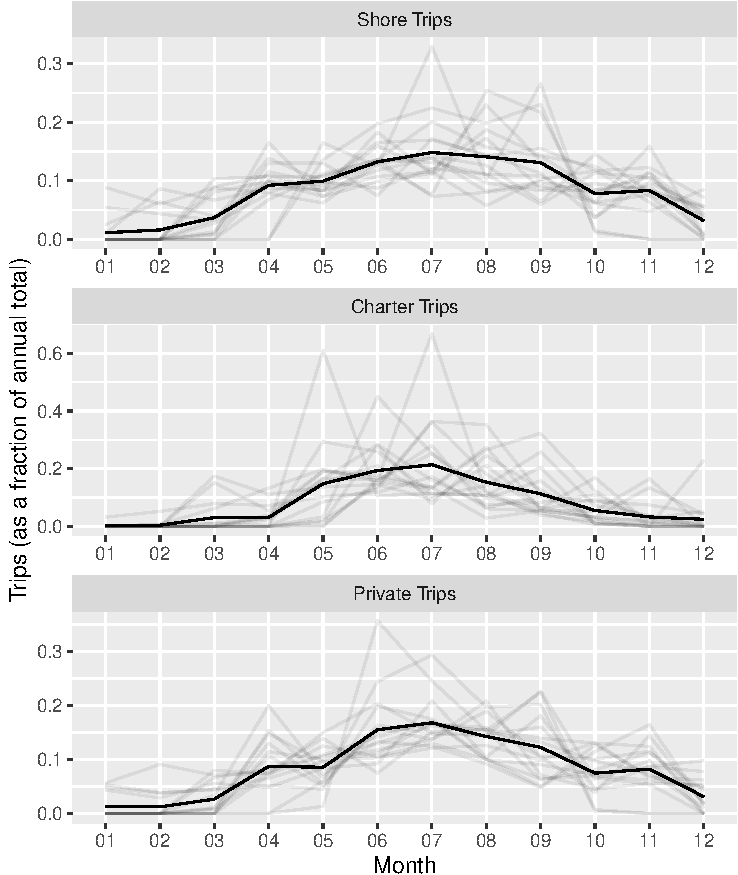
\includegraphics{C19PolicyRec_files/figure-latex/trips-seasonality-plot-1} 
}
\caption{2019 Monthly Marine Sportfishing Trips by State, relative to annual total. }\label{fig:trips-seasonality-plot}
\end{figure}

\begin{figure}

{\centering 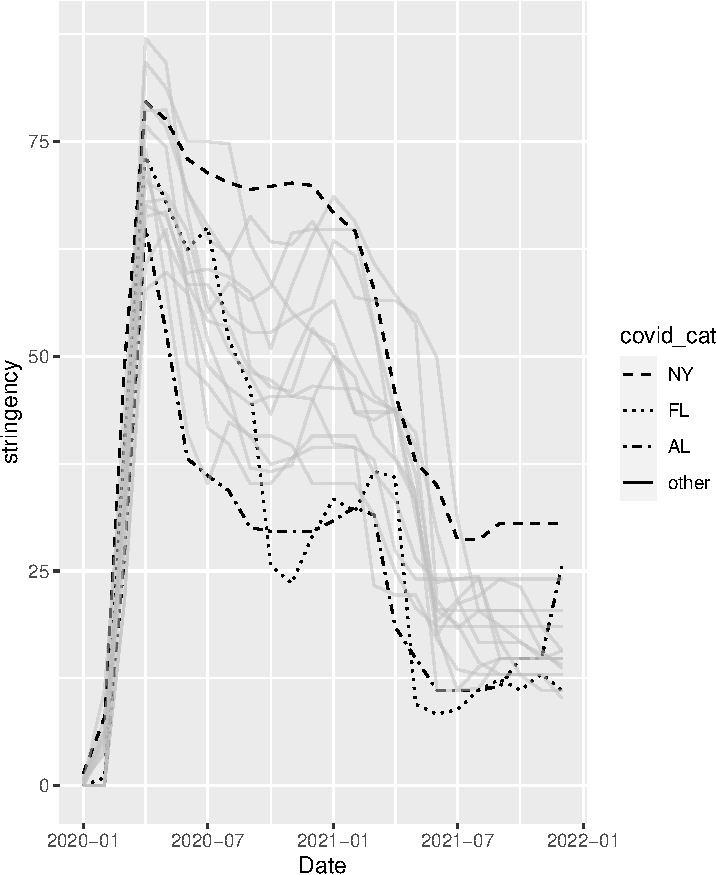
\includegraphics{C19PolicyRec_files/figure-latex/pString-1} 

}

\caption{Monthly 2020 stringency Index by State}\label{fig:pString}
\end{figure}

\begin{figure}
\centering
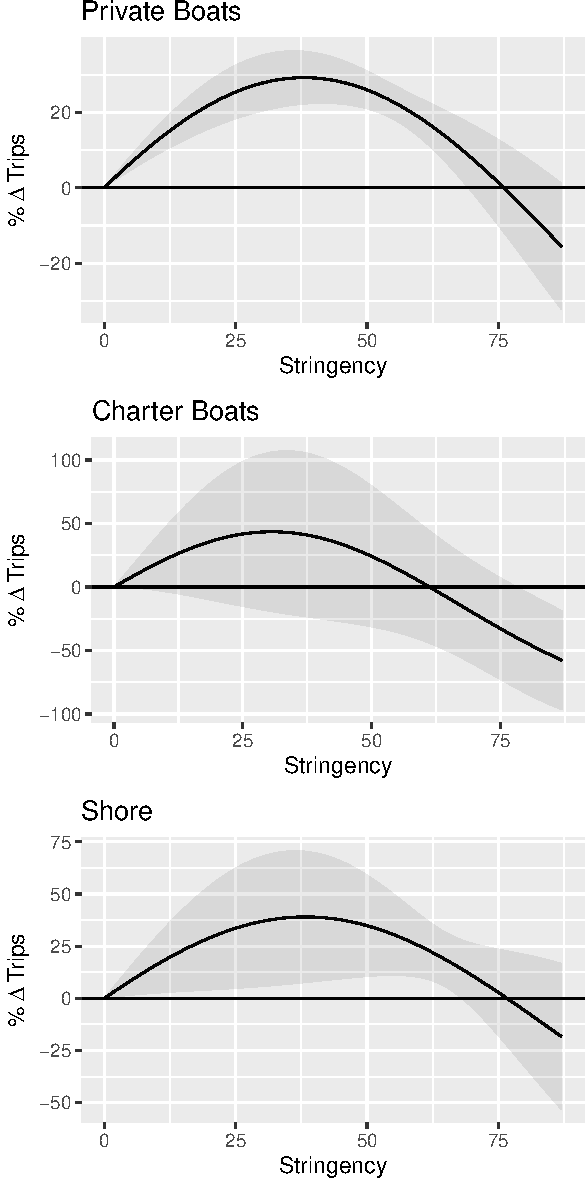
\includegraphics{C19PolicyRec_files/figure-latex/tripStringRel-1.pdf}
\caption{Predicted Percentage Change in Trips as a Function of the
Stringency Index}\label{fig:tripStringRel}
\end{figure}

\end{document}
